\section{MCP tool definitions, enforcement and transports}
\label{sec:mcpcontract}

\Cref{sec:mcp} followed one tool call from the user to an MCP server and back. This section reads
the tool definition that a server publishes and asks which parts of Lecture~4's tool contract MCP
enforces and which it leaves to trust. The distinction matters because a hostile server can falsify
any part that rests on trust (\cref{sec:attacks}). The section then follows the messages over stdio
and Streamable HTTP and asks what happens when a reply never arrives, the failure that Lecture~4
studied as a retried request.

\subsection{The SDK generates the tool definition}
\label{sec:mcpcontract-sdk}

A server's author writes an ordinary typed Python function, and the official Python SDK, the library
introduced in \cref{sec:mcp}, generates the whole MCP tool definition from it
\citep{mcp-python-sdk}. The course's \demoref{edit} tool replaces one exact occurrence of the text
\demoref{old} with the text \demoref{new} in the file at \demoref{path}. It refuses the call when
\demoref{old} does not appear exactly once.

\Cref{lst:mcpcontract-decorator} shows \demoref{edit} from the edit server of \cref{sec:mcp}. In
\cref{sec:mcp}, the SDK's tool decorator took no arguments. In \cref{lst:mcpcontract-decorator}, it
receives arguments that set the tool's name, title, description and annotations, and one that
requires an output schema.

\noindent\begin{minipage}{\linewidth}
\begin{lstlisting}[basicstyle=\ttfamily\footnotesize, caption={Illustrative server code: the
\texttt{edit} tool with explicit arguments to the SDK's tool decorator.},
label=lst:mcpcontract-decorator]
mcp = MCPServer("workspace")

class EditResult(TypedDict):
    path: str
    replaced: int

@mcp.tool(
    name="edit",
    title="Edit a workspace file",
    description="Replace one exact occurrence "
                "of old with new.",
    annotations=ToolAnnotations(
        read_only_hint=False, destructive_hint=True,
        idempotent_hint=False, open_world_hint=False),
    structured_output=True,
)
def edit(path: str, old: str, new: str) -> EditResult:
    """Replace one exact occurrence of old with new."""
    ...
\end{lstlisting}
\end{minipage}

The object \demoref{mcp} is the server, and its \demoref{tool} decorator registers the function
below it as a tool. The body of the function, left out of the listing, performs the edit. The SDK reads each part of the definition from a part of this code:
\bi
\item \textbf{Name, title and description.} The decorator's \demoref{name}, \demoref{title} and
\demoref{description} set them. When the name or the description is omitted, the SDK takes the name
from the function's name and the description from its docstring.
\item \textbf{Input schema.} The SDK builds the input schema from the type hints of the parameters.
Each parameter becomes a property with its type, and a parameter without a default value becomes a
required property.
\item \textbf{Output schema.} An \textbf{output schema} is a JSON Schema that the tool's structured
content (\demoref{structuredContent}, \cref{sec:mcp}) must match. The SDK builds it from the
function's return type. For \demoref{edit}, the return type is \demoref{EditResult}, a typed
dictionary with a string \demoref{path} and an integer \demoref{replaced}, so the output schema
describes an object with those two fields. A typed dictionary, a Pydantic model or a dataclass
becomes an object schema in this way. A scalar type such as \demoref{int}, or a list, is wrapped in
an object with a single field, \demoref{result}.
\item \textbf{Annotations.} The \demoref{ToolAnnotations} object carries the \textbf{tool
annotations}, four optional true-or-false hints about the tool's side effects, which
\cref{sec:mcpcontract-annotations} defines one by one. Python spells their names in snake case
(\demoref{read\_only\_hint}), and the definition sent to clients spells them in camel case
(\demoref{readOnlyHint}).
\ei

The output schema is optional. With \demoref{structured\_output=True}, as here, the SDK reports an
error when it registers a tool whose return type yields no schema. With
\demoref{structured\_output=False}, it publishes no output schema.

\Cref{lst:mcpcontract-definition} shows the definition that the server returns when a client sends
\demoref{tools/list}. The server's author wrote none of this JSON. The decorator can also attach
display icons and a \demoref{\_meta} object of further metadata, which both listings leave out.

\noindent\begin{minipage}{\linewidth}
\begin{lstlisting}[basicstyle=\ttfamily\footnotesize, caption={The tool definition that the SDK
generates from the code of \cref{lst:mcpcontract-decorator}, abridged by leaving out the titles
that the SDK adds to each schema and to every property.},
label=lst:mcpcontract-definition]
{
  "name": "edit",
  "title": "Edit a workspace file",
  "description":
    "Replace one exact occurrence of old with new.",
  "inputSchema": {
    "type": "object",
    "properties": {"path": {"type": "string"},
                   "old":  {"type": "string"},
                   "new":  {"type": "string"}},
    "required": ["path", "old", "new"]},
  "outputSchema": {
    "type": "object",
    "properties": {"path": {"type": "string"},
                   "replaced": {"type": "integer"}},
    "required": ["path", "replaced"]},
  "annotations": {
    "readOnlyHint": false, "destructiveHint": true,
    "idempotentHint": false, "openWorldHint": false}
}
\end{lstlisting}
\end{minipage}

Most fields of the definition carry one of the five parts of the tool contract (\cref{sec:recap}),
and the rest serve display:
\bi
\item \textbf{Purpose.} The \demoref{title} is a human-readable name for display, and the
\demoref{description} tells the model what the tool does.
\item \textbf{Arguments.} The \demoref{inputSchema} lists the arguments, their types and which of
them are required.
\item \textbf{Results and errors.} The \demoref{outputSchema} describes the structured content of a
result. A failure is reported in the result itself through \demoref{isError} (\cref{sec:mcp}).
\item \textbf{Side effects.} The \demoref{annotations} hold the four side-effect hints.
\item \textbf{Display and metadata.} The \demoref{icons} are images that a client can show in its
user interface, and \demoref{\_meta} holds any further metadata. Neither describes what the tool
does when it runs.
\ei

The host obtains this definition through \demoref{tools/list} and only reads it. Nothing in the
definition lets the host check that the code behind it does what the definition says. The host also
passes on only part of it. The model receives the name, the description and the input schema,
converted into a native tool definition (\cref{sec:mcp}). The title, the output schema, the
annotations, the icons and \demoref{\_meta} stay with the host.

\subsection{Which parts of the contract MCP enforces}
\label{sec:mcpcontract-enforce}

MCP gives an enforcer only to the shapes of a tool's arguments and results.
\Cref{tab:mcpcontract-enforce} places each of the five parts of the tool contract next to the MCP
field that carries it and the party that the specification makes responsible for it
\citep{mcp-spec-2026}. The rows for purpose and for side effects name no enforcer, and the row for
execution constraints names no field.

\begin{table}[htbp]
  \caption{The parts of a tool contract, the MCP fields that carry them, and who enforces each
  part. Only the input schema and the output schema have an enforcer.}
  \label{tab:mcpcontract-enforce}
  \begin{adjustbox}{width=\linewidth}\begin{tabularx}{\linewidth}{L{0.23\linewidth}L{0.35\linewidth}X}
    \toprule
    \textbf{Contract part} & \textbf{MCP field} & \textbf{Who enforces it} \\
    \midrule
    \textbf{Purpose} & \demoref{description}, \demoref{title} & No one. The model reads it. \\
    \textbf{Arguments} & \demoref{inputSchema} & The server, which must validate all tool inputs. \\
    \textbf{Results and errors} & \demoref{outputSchema}, \demoref{content}, \demoref{structuredContent}, \demoref{isError} & The server must return structured content that conforms to the output schema, and the client should validate it. No one checks meaning. \\
    \textbf{Side effects} & \demoref{annotations} & No one. They are hints, untrusted unless the server is trusted. \\
    \textbf{Execution constraints} & No field & The code of the host and the server. \\
    \bottomrule
  \end{tabularx}\end{adjustbox}
\end{table}

Each row has the following meaning:
\bi
\item \textbf{Purpose.} The description is text that the model reads when it chooses a tool. No
party checks that it is true, and the host forwards it as the server's author wrote it.
\item \textbf{Arguments.} The server must validate all tool inputs, whose shape the input
schema describes. A call with a missing or ill-typed argument returns a tool execution error, a result with
\demoref{isError} set to true (\cref{sec:mcp}).
\item \textbf{Results and errors.} When a tool declares an output schema, the server must return
structured content that conforms to it, and the client should validate it. These checks cover only
the shape of a result. A result can report one replacement in the correct format even
when the tool edited the wrong line, just as Lecture~4 found that a call can match its argument
schema and still name the wrong file.
\item \textbf{Side effects.} The annotations are hints. Clients must treat them as untrusted unless
they come from a trusted server.
\item \textbf{Execution constraints.} The specification has no field for constraints such as
timeouts, quotas or confinement to a directory. The code of the host and the server enforces them.
In our example, the edit server's own code refuses paths outside its workspace. A client should set
its own timeout for each request it sends.
\ei

MCP thus divides a tool's contract into checked parts and trusted parts. Code checks the shapes of
arguments and results. The description and the annotations are statements by the server's author,
which the host must take on trust. Execution constraints hold only where someone wrote code to
enforce them, and the definition does not tell the host whether anyone did.

The trusted parts matter because the model reads one of them. A host that connects to a server it
does not trust passes the model a description that no one has verified, and the model treats it as
an account of the tool. \Cref{sec:attacks} studies attacks that place instructions in this text.

\subsection{Annotations are hints}
\label{sec:mcpcontract-annotations}

Tool annotations describe a tool's side effects, but nothing binds a server to them, so a client may
rely on them only when it trusts the server. Each of the four hints has a meaning and a default that
applies when the server omits it:
\bi
\item \textbf{\demoref{readOnlyHint}.} If true, the tool does not modify its environment. The
default is false.
\item \textbf{\demoref{destructiveHint}.} If true, the tool may perform destructive updates. If
false, it performs only additive updates. The default is true.
\item \textbf{\demoref{idempotentHint}.} If true, calling the tool repeatedly with the same
arguments has no additional effect on its environment. The default is false.
\item \textbf{\demoref{openWorldHint}.} If true, the tool may interact with an open world of
external entities. The default is true.
\ei
Each default assumes the riskier behavior. A tool that declares nothing is treated as one that may
modify its environment, destroy data, repeat its effect when called again, and reach outside
systems.

The annotations of \cref{lst:mcpcontract-definition} fit \demoref{edit}. The tool modifies files, so
\demoref{readOnlyHint} is false. It overwrites text instead of only adding text, so
\demoref{destructiveHint} is true. It reaches no system outside the workspace, so
\demoref{openWorldHint} is false.

Because the server's author chooses the hints and nothing checks them, a hint can misdescribe the
tool. The same holds for the display \demoref{title} that the annotations may also carry.

\begin{definition}[Tool annotations are hints]
\label{def:mcpcontract-annotations}
``[A]ll properties in \texttt{ToolAnnotations} are hints. They are not guaranteed to provide a
faithful description of tool behavior (including descriptive properties like \texttt{title}).
Clients should never make tool use decisions based on \texttt{ToolAnnotations} received from
untrusted servers.'' \citep{mcp-spec-2026}
\end{definition}

A tool use decision is any choice a client makes about calling a tool. A host could, for example,
ask for the user's consent before every call to a destructive tool but only once for a tool marked
read-only. With an untrusted server it should not do so, because a hostile server can mark a
destructive tool as read-only.

Even an honest hint can be too coarse. Lecture~4 called a request idempotent when repeating it has
the same effect as executing it once. The hint \demoref{idempotentHint} is one flag for the whole
tool, whereas whether a repeated call has an additional effect can depend on the arguments.
\Cref{lst:mcpcontract-idem} shows two pairs of identical calls to \demoref{edit} on constructed
files. Each file contains the text to be replaced exactly once before the first call of its pair.

\noindent\begin{minipage}{\linewidth}
\begin{lstlisting}[basicstyle=\ttfamily\footnotesize, caption={Illustrative calls: the same
\texttt{edit} call made twice, for two sets of arguments.}, label=lst:mcpcontract-idem]
# src/parse.py contains "i <= n" once
edit("src/parse.py", "i <= n", "i < n")
    # changes the file
edit("src/parse.py", "i <= n", "i < n")
    # refused: old no longer appears

# src/limit.py contains "count" once
edit("src/limit.py", "count", "count + 1")
    # changes the file
edit("src/limit.py", "count", "count + 1")
    # changes it again
\end{lstlisting}
\end{minipage}

In the first pair, the first call replaces \demoref{i <= n} with \demoref{i < n}. The repeated call
finds no \demoref{i <= n} in the file, so \demoref{edit} refuses it, and the file does not change
again. For these arguments, \demoref{edit} behaves idempotently.

In the second pair, the new text \demoref{count + 1} contains the old text \demoref{count}. After
the first call, \demoref{count} still appears exactly once, inside \demoref{count + 1}. The repeated
call therefore succeeds, and the file then contains \demoref{count + 1 + 1}. For these arguments,
\demoref{edit} is not idempotent.

A single flag cannot describe both cases. The server marks \demoref{edit} with
\demoref{idempotentHint} false, which is correct for the tool as a whole. The flag says nothing
about whether one particular repeated call is safe, and that is the question a client faces when it
sends a request again (\cref{sec:mcpcontract-retry}).

\subsection{Every request stands on its own}
\label{sec:mcpcontract-stateless}

MCP is a \textbf{stateless protocol}: every request carries everything needed to process it, so a
server may not rely on earlier requests.

\begin{definition}[Stateless protocol]
\label{def:mcpcontract-stateless}
``The Model Context Protocol (MCP) is a stateless protocol: all the information needed to process a
request is contained in the request itself. A server processes each request independently; no state
should be inferred from previous requests, even those on the same connection or stream.''
\citep{mcp-spec-2026}
\end{definition}

Every request therefore carries its protocol version and the client's capabilities, the optional
features that the client itself supports. \Cref{lst:mcpcontract-meta} shows where they travel: in a
\demoref{\_meta} object inside the parameters of the request, one key for each value. The protocol
version and the client capabilities are required on every request. The client's name and version
are optional, although clients should send them.

\noindent\begin{minipage}{\linewidth}
\begin{lstlisting}[basicstyle=\ttfamily\footnotesize, caption={The metadata carried in the
parameters of every request, as in the specification's own example.}, label=lst:mcpcontract-meta]
"_meta": {
  "io.modelcontextprotocol/protocolVersion": "2026-07-28",
  "io.modelcontextprotocol/clientCapabilities": {},
  "io.modelcontextprotocol/clientInfo":
      {"name": "ExampleClient", "version": "1.0.0"}
}
\end{lstlisting}
\end{minipage}

A server must not use earlier requests on the same connection to learn any of these values.
Earlier revisions of MCP exchanged them once, in an opening handshake that started a protocol
session, a context on which later requests relied. Revision 2026-07-28 has no handshake and no
session. The server accepts or rejects each request on its own, according to the protocol version
that the request names. An open connection, such as the standard streams of a server process, may
carry unrelated requests one after another, and the server must not treat it as one conversation.

Some tools need state that spans several calls, such as a shopping basket that one call creates and
later calls fill. Such state travels as a \textbf{handle}: an explicit identifier that one call
returns and later calls pass back as an ordinary argument. A call that creates a basket, for
example, returns an identifier such as \demoref{basket\_id}, and each later call that adds an item
passes it. The server stores the basket under that identifier and looks it up on each call, so the
state lives with the handle. The connection plays no part in it.

Statelessness has a consequence for failures. Because each request is complete in itself, a client
can send any request again, to the same server process or to a new one, and the server processes
the copy as an independent request. The protocol also gives the server nothing with which to
recognize the copy as a repeat (\cref{sec:mcpcontract-retry}).

\subsection{The stdio transport}
\label{sec:mcpcontract-stdio}

Over stdio, each message is one line of JSON, and the newline at the end of the line ends the
message. As in \cref{sec:mcp}, stdio is the transport in which the client starts the server as a
subprocess and the two exchange messages over the subprocess's standard input and output. Any
transport that sends messages over a stream of bytes needs \textbf{framing}, a rule by which the
receiver finds where one message ends and the next begins. On stdio, the rule is the newline
\citep{mcp-spec-2026}:
\bi
\item \textbf{Requests.} The client writes each request to the server's standard input as JSON
containing no raw newline, followed by one newline.
\item \textbf{Replies.} The server writes each response to its standard output in the same way, and
the client reads one line per message. All replies arrive on this one stream, so the client matches
each response to its request by the request ID.
\item \textbf{Newlines in values.} A line break inside a string value is written as the escape
sequence \demoref{\textbackslash n}, a backslash followed by the letter n. The newline after a
message is therefore the only raw newline it contains.
\item \textbf{Logs.} The server may write log messages to its standard error stream. It must not
write anything to standard output that is not a valid MCP message.
\ei

The rule about logs follows from the framing. The client reads every line on standard output as a
message, so a line of debugging output printed there would reach the client as a malformed message.

The framing rule uses only the newline, so it does not depend on the standard streams. The same
format works over any reliable two-way stream of bytes, such as a Unix socket or a TCP connection.

\subsection{The Streamable HTTP transport}
\label{sec:mcpcontract-http}

Over Streamable HTTP, every message from the client is a new HTTP POST request to the server's
endpoint, the single URL path at which it accepts MCP messages (\cref{sec:mcp}). The body of each
POST is one JSON-RPC message, and its headers repeat the parts of the message that matter for
routing \citep{mcp-spec-2026}. \Cref{lst:mcpcontract-post} shows the request line and headers of a
\demoref{tools/call} request for \demoref{edit}.

\noindent\begin{minipage}{\linewidth}
\begin{lstlisting}[basicstyle=\ttfamily\footnotesize, caption={The request line and headers of a
\texttt{tools/call} request over Streamable HTTP. The body, not shown, is the JSON-RPC request.},
label=lst:mcpcontract-post]
POST /mcp HTTP/1.1
Content-Type: application/json
Accept: application/json, text/event-stream
MCP-Protocol-Version: 2026-07-28
Mcp-Method: tools/call
Mcp-Name: edit
\end{lstlisting}
\end{minipage}

The headers have the following roles:
\bi
\item \textbf{\demoref{Accept}.} The client must list both \demoref{application/json} and
\demoref{text/event-stream}, because the server may answer in either form.
\item \textbf{\demoref{MCP-Protocol-Version}.} Every POST must carry this header, and its value must
match the protocol version in the request's \demoref{\_meta}.
\item \textbf{\demoref{Mcp-Method} and \demoref{Mcp-Name}.} \demoref{Mcp-Method} repeats the method
and is required on all requests. \demoref{Mcp-Name} repeats the name of the tool or MCP prompt, or
the URI of the resource, and is required on \demoref{tools/call}, \demoref{resources/read} and
\demoref{prompts/get}.
\ei
The headers repeat what the body already says so that intermediaries such as load balancers can
route and inspect a request without parsing its body.

The server answers a request in one of two forms, and the client must support both. It returns
either a single JSON object, marked \demoref{Content-Type: application/json}, or a stream of
\textbf{server-sent events} (SSE), an HTTP response that stays open and delivers a sequence of
events, marked \demoref{Content-Type: text/event-stream} (\cref{sec:mcpcontract-sse}). A reply as
one JSON object is the JSON-RPC response itself, with the same request ID as the request.

The server must also validate the \demoref{Origin} header on every incoming connection. A browser
adds this header to many of the requests that a web page sends, including every POST request, and
it names the origin of that page: the scheme, host and port of its address. The check prevents DNS rebinding, an attack through which a
public web page reaches a server running on the user's own machine. \Cref{sec:inspector} studies a
local component that lacked such checks.

\subsection{Progress and cancellation over server-sent events}
\label{sec:mcpcontract-sse}

\begin{figure*}[tb]
  \centering
  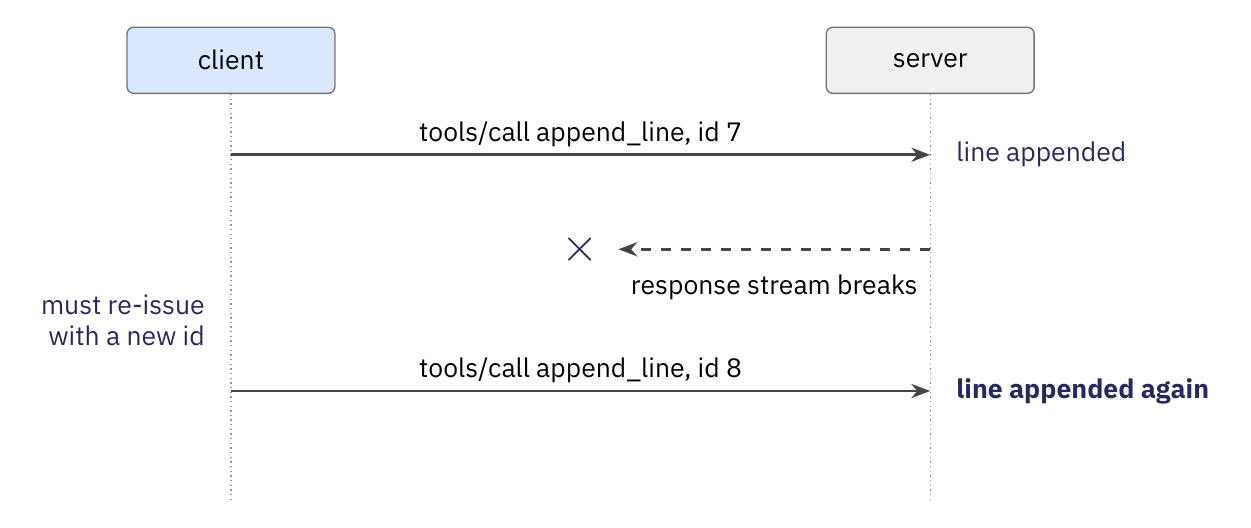
\includegraphics[width=0.75\textwidth]{figures/deck/09311a23b9.png}
  \caption{A broken response stream and the request sent again. The first call appends a line, its
  response stream breaks, and the client re-issues the call with a new request ID, so the server
  appends the line a second time. The tool \texttt{append\_line} is illustrative.}
  \label{fig:mcpcontract-retry}
\end{figure*}

When the server answers with a stream of events, it can report progress before it sends the result.
In the replies of the official Python SDK, each SSE event consists of an event line
(\demoref{event: message}), a data line that carries one JSON-RPC message, and a blank line that
ends the event (\cref{lst:mcpcontract-sse}). The specification itself does not require the event
line.

\noindent\begin{minipage}{\linewidth}
\begin{lstlisting}[basicstyle=\ttfamily\footnotesize, caption={The shape of an SSE reply to a
\texttt{tools/call} request: a progress notification, then the result. The angle brackets stand
for the JSON-RPC messages.}, label=lst:mcpcontract-sse]
HTTP/1.1 200 OK
Content-Type: text/event-stream

event: message
data: <notifications/progress message>

event: message
data: <JSON-RPC response with id 2>
\end{lstlisting}
\end{minipage}

A \textbf{progress notification} is a notification, sent on the stream before the result, that
reports how far the work on a request has come. A client asks for such reports by placing a
\textbf{progress token} in the request's \demoref{\_meta}. The token is an identifier that each
progress notification repeats, so that the client knows which request a report describes. In
\cref{lst:mcpcontract-sse}, the first event carries a progress notification and the second carries
the result.

The specification sets the following rules for such a stream \citep{mcp-spec-2026}:
\bi
\item \textbf{Related notifications only.} The server may send notifications before the final
response, and they must relate to the request that opened the stream.
\item \textbf{No requests.} The server must not send requests of its own on the stream.
\item \textbf{End of the stream.} The final response should end the stream.
\item \textbf{Closing means cancelling.} If the stream closes before the final response, the server
must treat the closing as cancellation of the request.
\ei

\textbf{Cancellation} means abandoning a request before its result arrives. On Streamable HTTP, a
client cancels a request by closing the request's stream, and the server should then stop the work.
The server treats a closed stream as cancellation whether the client closed it on purpose or the
connection broke. In either case, the server may already have finished the work. On stdio, which
has no stream per request, the client instead sends a \demoref{notifications/cancelled}
notification that names the request's ID.

\subsection{A broken stream forces a new request}
\label{sec:mcpcontract-retry}

A response stream that breaks before the result arrives loses the request, and the client must send
it again: ``A broken response stream loses the in-flight request; clients MUST re-issue it as a new
request with a new request ID'' \citep{mcp-spec-2026}. An in-flight request is one that has been
sent and not yet answered. Because every request is self-contained
(\cref{sec:mcpcontract-stateless}), the client can send it again in full.

Streams cannot be resumed, and the server does not redeliver a result once the stream that should
have carried it is gone. On stdio, the same loss happens when the server process exits
unexpectedly. The requests in flight are lost, and the client can send them again to a new server
process.

The protocol's own repeats of a request also use new IDs. When a server needs more input before it
can finish, it answers with an \demoref{input\_required} result (\cref{sec:mcp}). The client then
sends the original request again with the answer added, and the request ID of the repeat must
differ from that of the first request. Every repeat of a request, whether the protocol's own or one
after a broken stream, therefore carries a new ID. The ID cannot tell the server that two requests
ask for the same operation.

MCP also lacks the means by which a server could recognize a repeat or bound the work it does:
\bi
\item \textbf{No idempotency key.} Lecture~4 defined an idempotency key as an identifier that a
request carries so that the receiver can detect a duplicate and decline to repeat its effect. MCP
defines no such field for \demoref{tools/call}. The only related field is \demoref{idempotentHint},
which is untrusted and covers the whole tool (\cref{sec:mcpcontract-annotations}).
\item \textbf{No deduplication.} The server is not required to detect that two requests ask for the
same operation.
\item \textbf{No deadline.} A \textbf{deadline} is a time limit carried in the request, after which the
work is no longer wanted. MCP requests carry none. The specification asks implementations to set
timeouts for all the requests they send, so each side keeps its own timeout. A server therefore
learns that a client has stopped waiting only if the client cancels the request, and it may finish
work after the client has given up.
\ei
The request ID therefore cannot serve as an idempotency key. An ID only has to differ from the IDs
of the sender's other requests that are still awaiting a reply.

\Cref{fig:mcpcontract-retry} shows what follows for a tool that is not idempotent. The illustrative
tool \demoref{append\_line} adds one line to a file. The client calls it with request ID 7, and the
server appends the line. The response stream breaks before the result reaches the client. The client
cannot tell whether the line was appended, and the rule requires it to re-issue the call with a new
ID, 8. The server sees an ordinary new request and appends the line a second time.

This is the failure that Lecture~4 studied as a retried request. There, the request with ID 7
applied a patch, its reply was lost, and the retry with ID 8 applied the patch again. Lecture~4
named the mechanism that prevents the second effect, the idempotency key. Under MCP, a tool that
needs one can declare it as an ordinary argument in its input schema, so the protection is left to
each tool's designer.

The protocol thus tells the client to send the request again and gives the server no way to
recognize the repeat. MCP therefore does not provide exactly-once semantics, in Lecture~4's sense of
a side effect that occurs once despite lost requests, lost replies or duplicate delivery.

\subsection{Who validates arguments and who resends a request}
\label{sec:mcpcontract-who}

The server must validate a tool's arguments, and the client must resend a request after a broken
stream. The reasons are as follows:
\bi
\item \textbf{Validating arguments.} The server must validate all tool inputs
\citep{mcp-spec-2026}. The host may check the arguments too, but the server cannot rely on
that check, because the host and the server do not trust each other (\cref{sec:mcp}). The
specification asks the client to validate the results that come back.
\item \textbf{Resending after a broken stream.} The client re-issues the request with a new request
ID. The server cannot redeliver the result, because streams cannot be resumed. The resend happens
entirely in the client, without the model.
\ei

\subsection*{Key points}
\bi
\item The official Python SDK generates an MCP tool definition from a typed function: the input
schema from the parameter type hints, the output schema from the return type, and, unless the
decorator sets them, the name from the function's name and the description from its docstring.
\item In MCP, only the shapes of a tool's arguments and results have an enforcer: the server must
validate all tool inputs and, when the tool declares an output schema, return structured content
that matches it, which the client should validate.
\item The description and the tool annotations have no enforcer and rest on trust in the server,
and MCP has no field for execution constraints, which exist only in the code of the host and the
server.
\item Tool annotations are hints that a client must treat as untrusted unless the server is trusted,
and \demoref{idempotentHint} is one flag for the whole tool although idempotency can depend on the
arguments.
\item MCP is stateless: every request carries its protocol version and client capabilities, a server
may not rely on earlier requests on a connection, and state that spans calls travels as an explicit
handle in the tool arguments.
\item On stdio a newline ends each message, and on Streamable HTTP each message from the client is a
new POST to one endpoint, whose server must validate the Origin header and may answer with an SSE stream that
carries progress notifications and whose closing cancels the request.
\item When a response stream breaks, the client must re-issue the request with a new request ID, and
because MCP has no idempotency key, deduplication or deadline, the server cannot recognize the
repeat, so a tool that is not idempotent can apply its effect twice.
\ei
